\documentclass{school}
\title{Lichtsetzung}
\subject{Medientechnik - Fotografie}
\author{Markus Reichl}

\begin{document}
\maketitle
\thispagestyle{fancy}

In der Fotografie werden verschiedene Lichtsetzungen verwendet, wobei sich bei der Aufnahme von Portraits besonders die folgenden 6 etabliert haben.

\section{Rembrandt}
\begin{figure}[h]
	\centering
	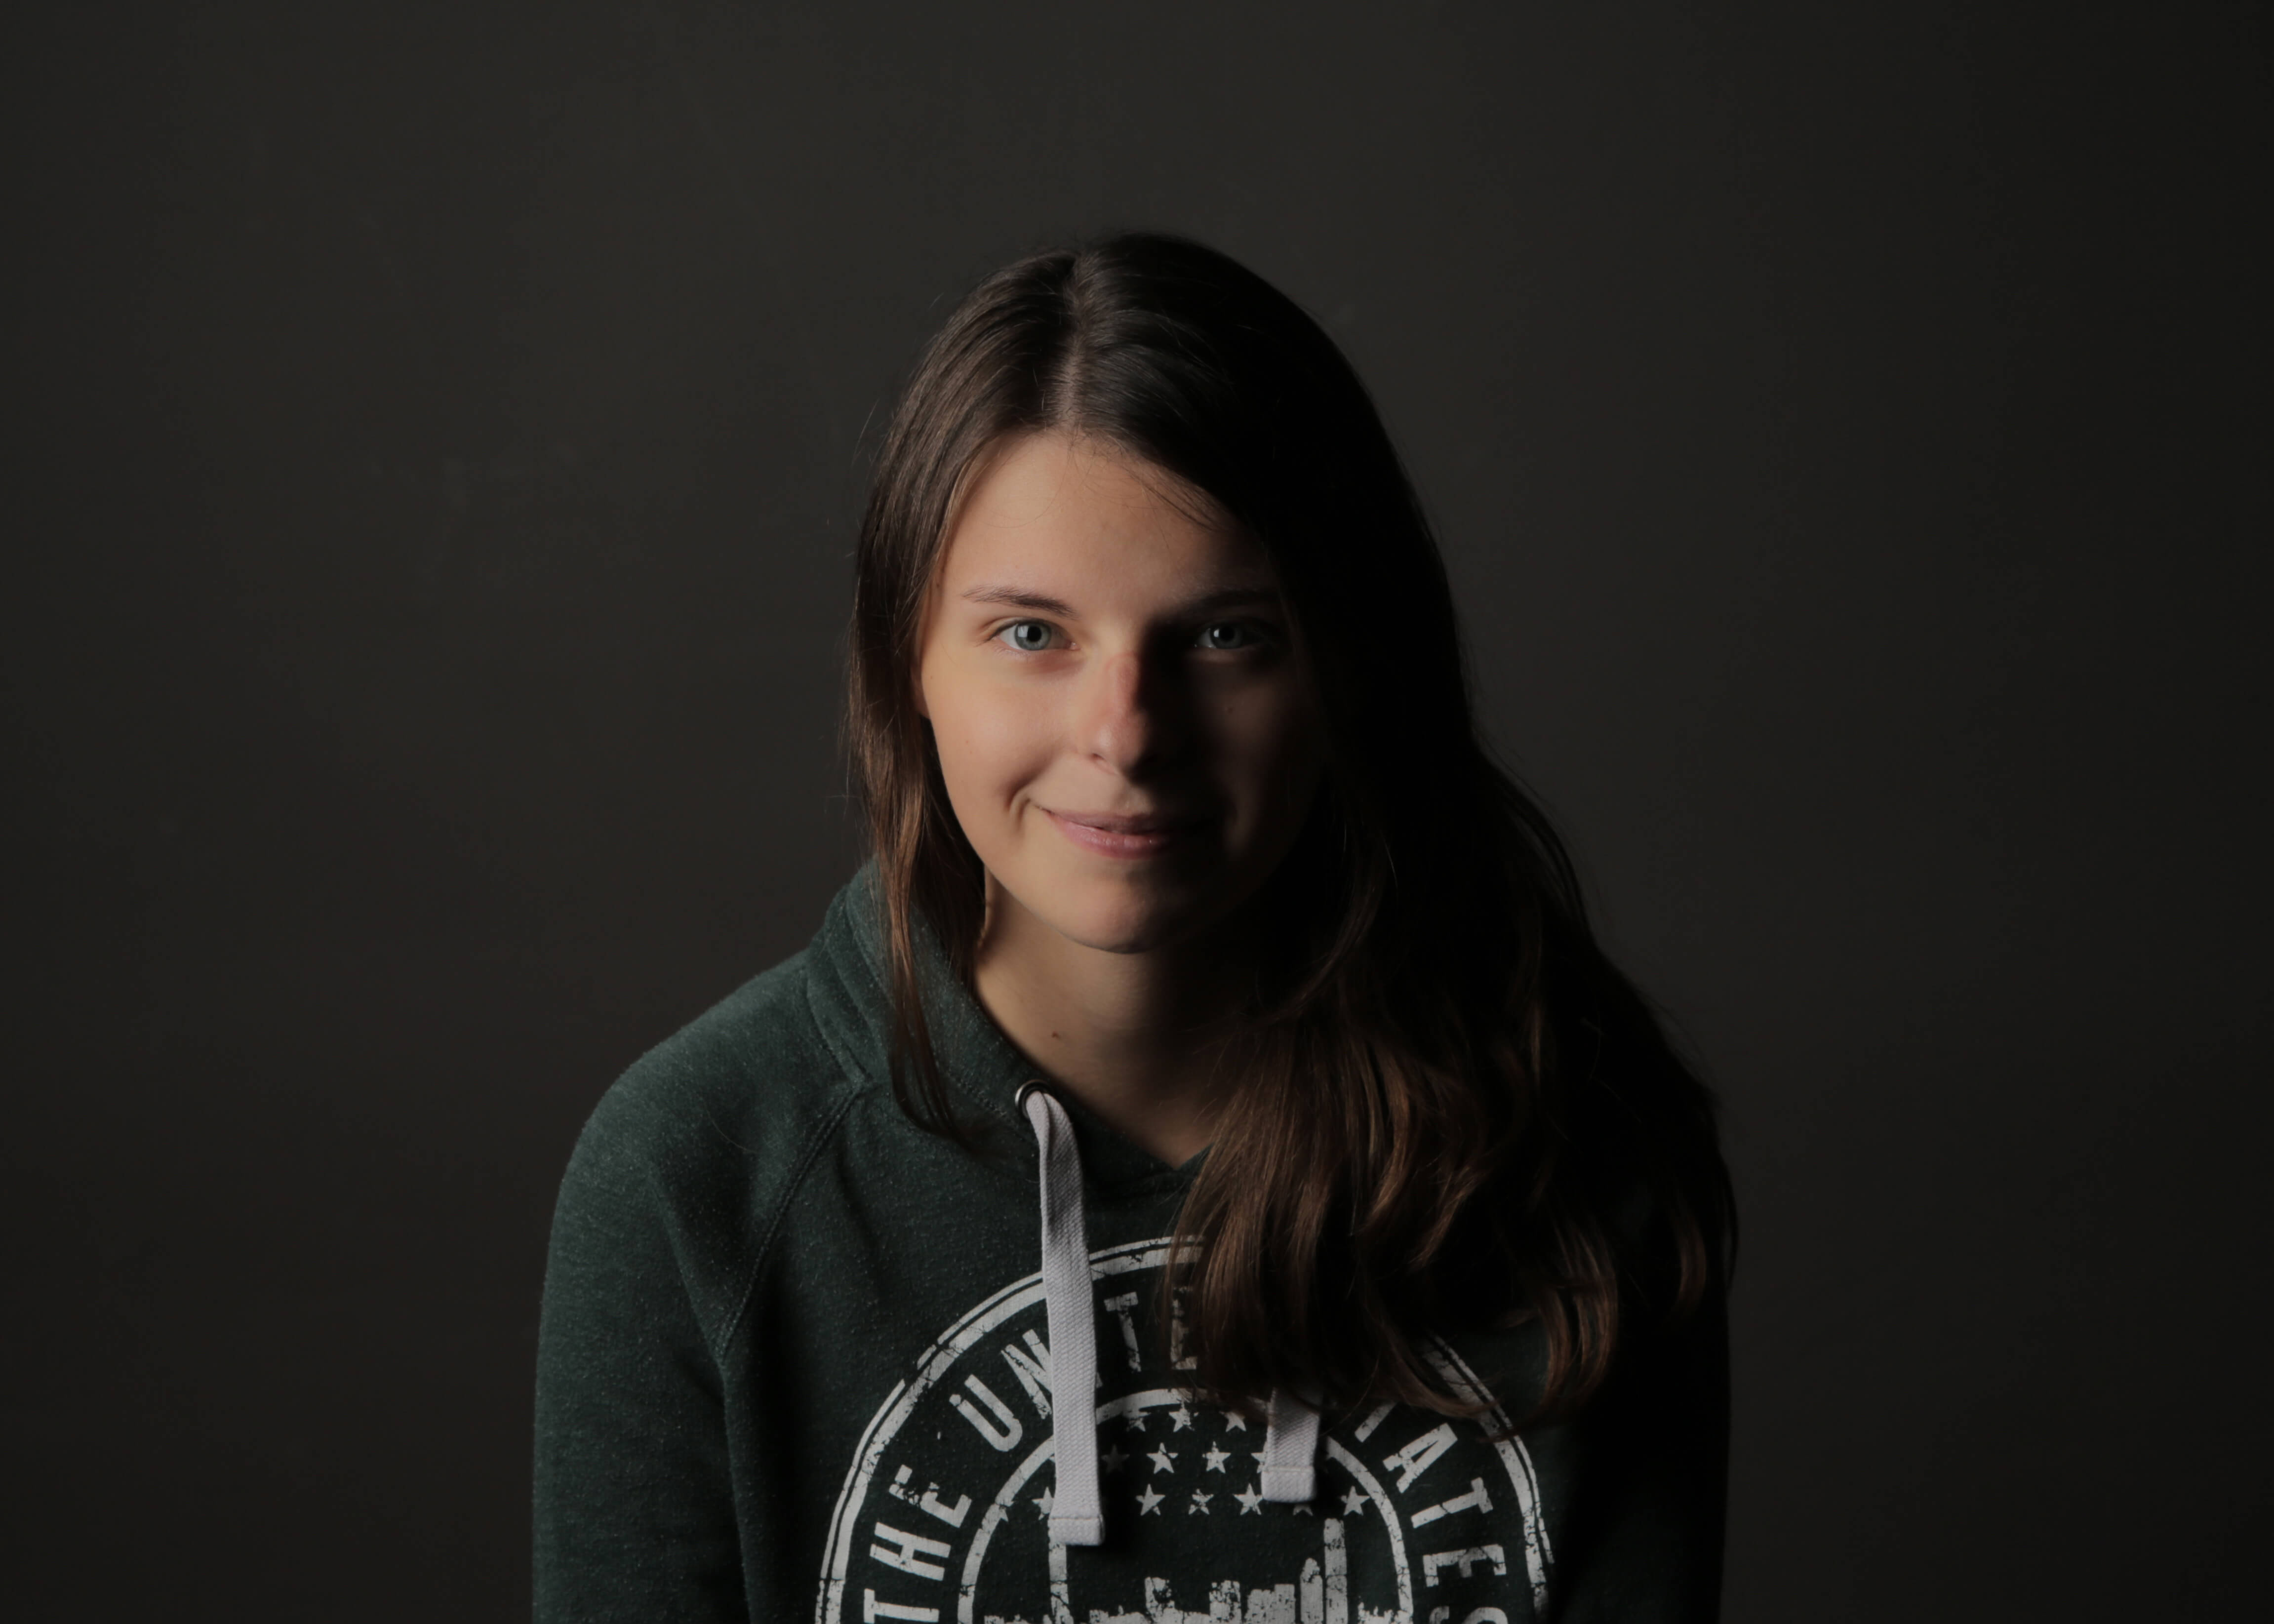
\includegraphics[height=5cm]{1-rembrandt.jpg}
	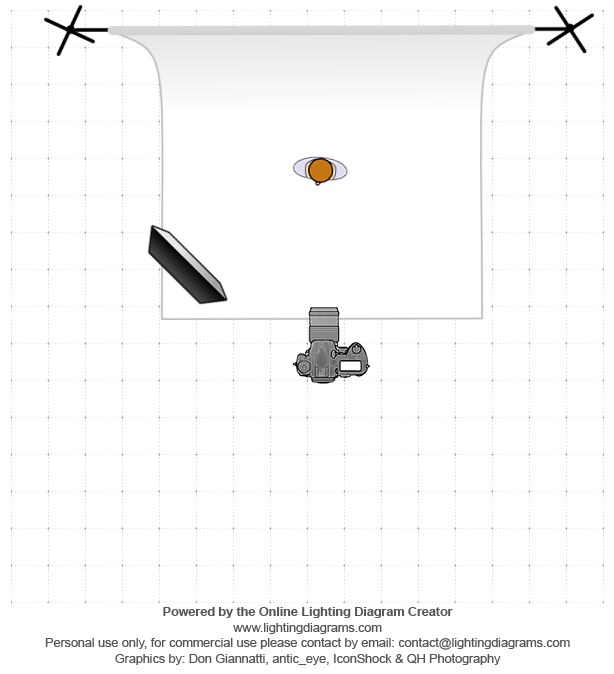
\includegraphics[height=5cm]{1-rembrandt-diagram.png}
	\caption{Rembrandt}
\end{figure}

"Beim Rembrandt-Licht ist die eine Seite des Kopfes ausgeleuchtet, während die andere Seite fast völlig im Dunkeln verschwindet...nur das charakteristische Lichtdreieck zeichnet sich, wenn die Lichtsetzung korrekt ist, auf der Schattenseite unter dem Auge ab."
$-$ Fotopraxis.at \cite{fp-rembrandt}
\\\\
Die Belichtung orientiert sich an Gemälden des Künstlers Rembrandt und wird gerne zusammen mit einem dunkleren Hintergrund verwendet. Das Licht ist dabei in einem 45 Grad Winkel zur und oberhalb der Person zu positionieren.

\newpage
\section{Seitlich}
\begin{figure}[h]
	\centering
	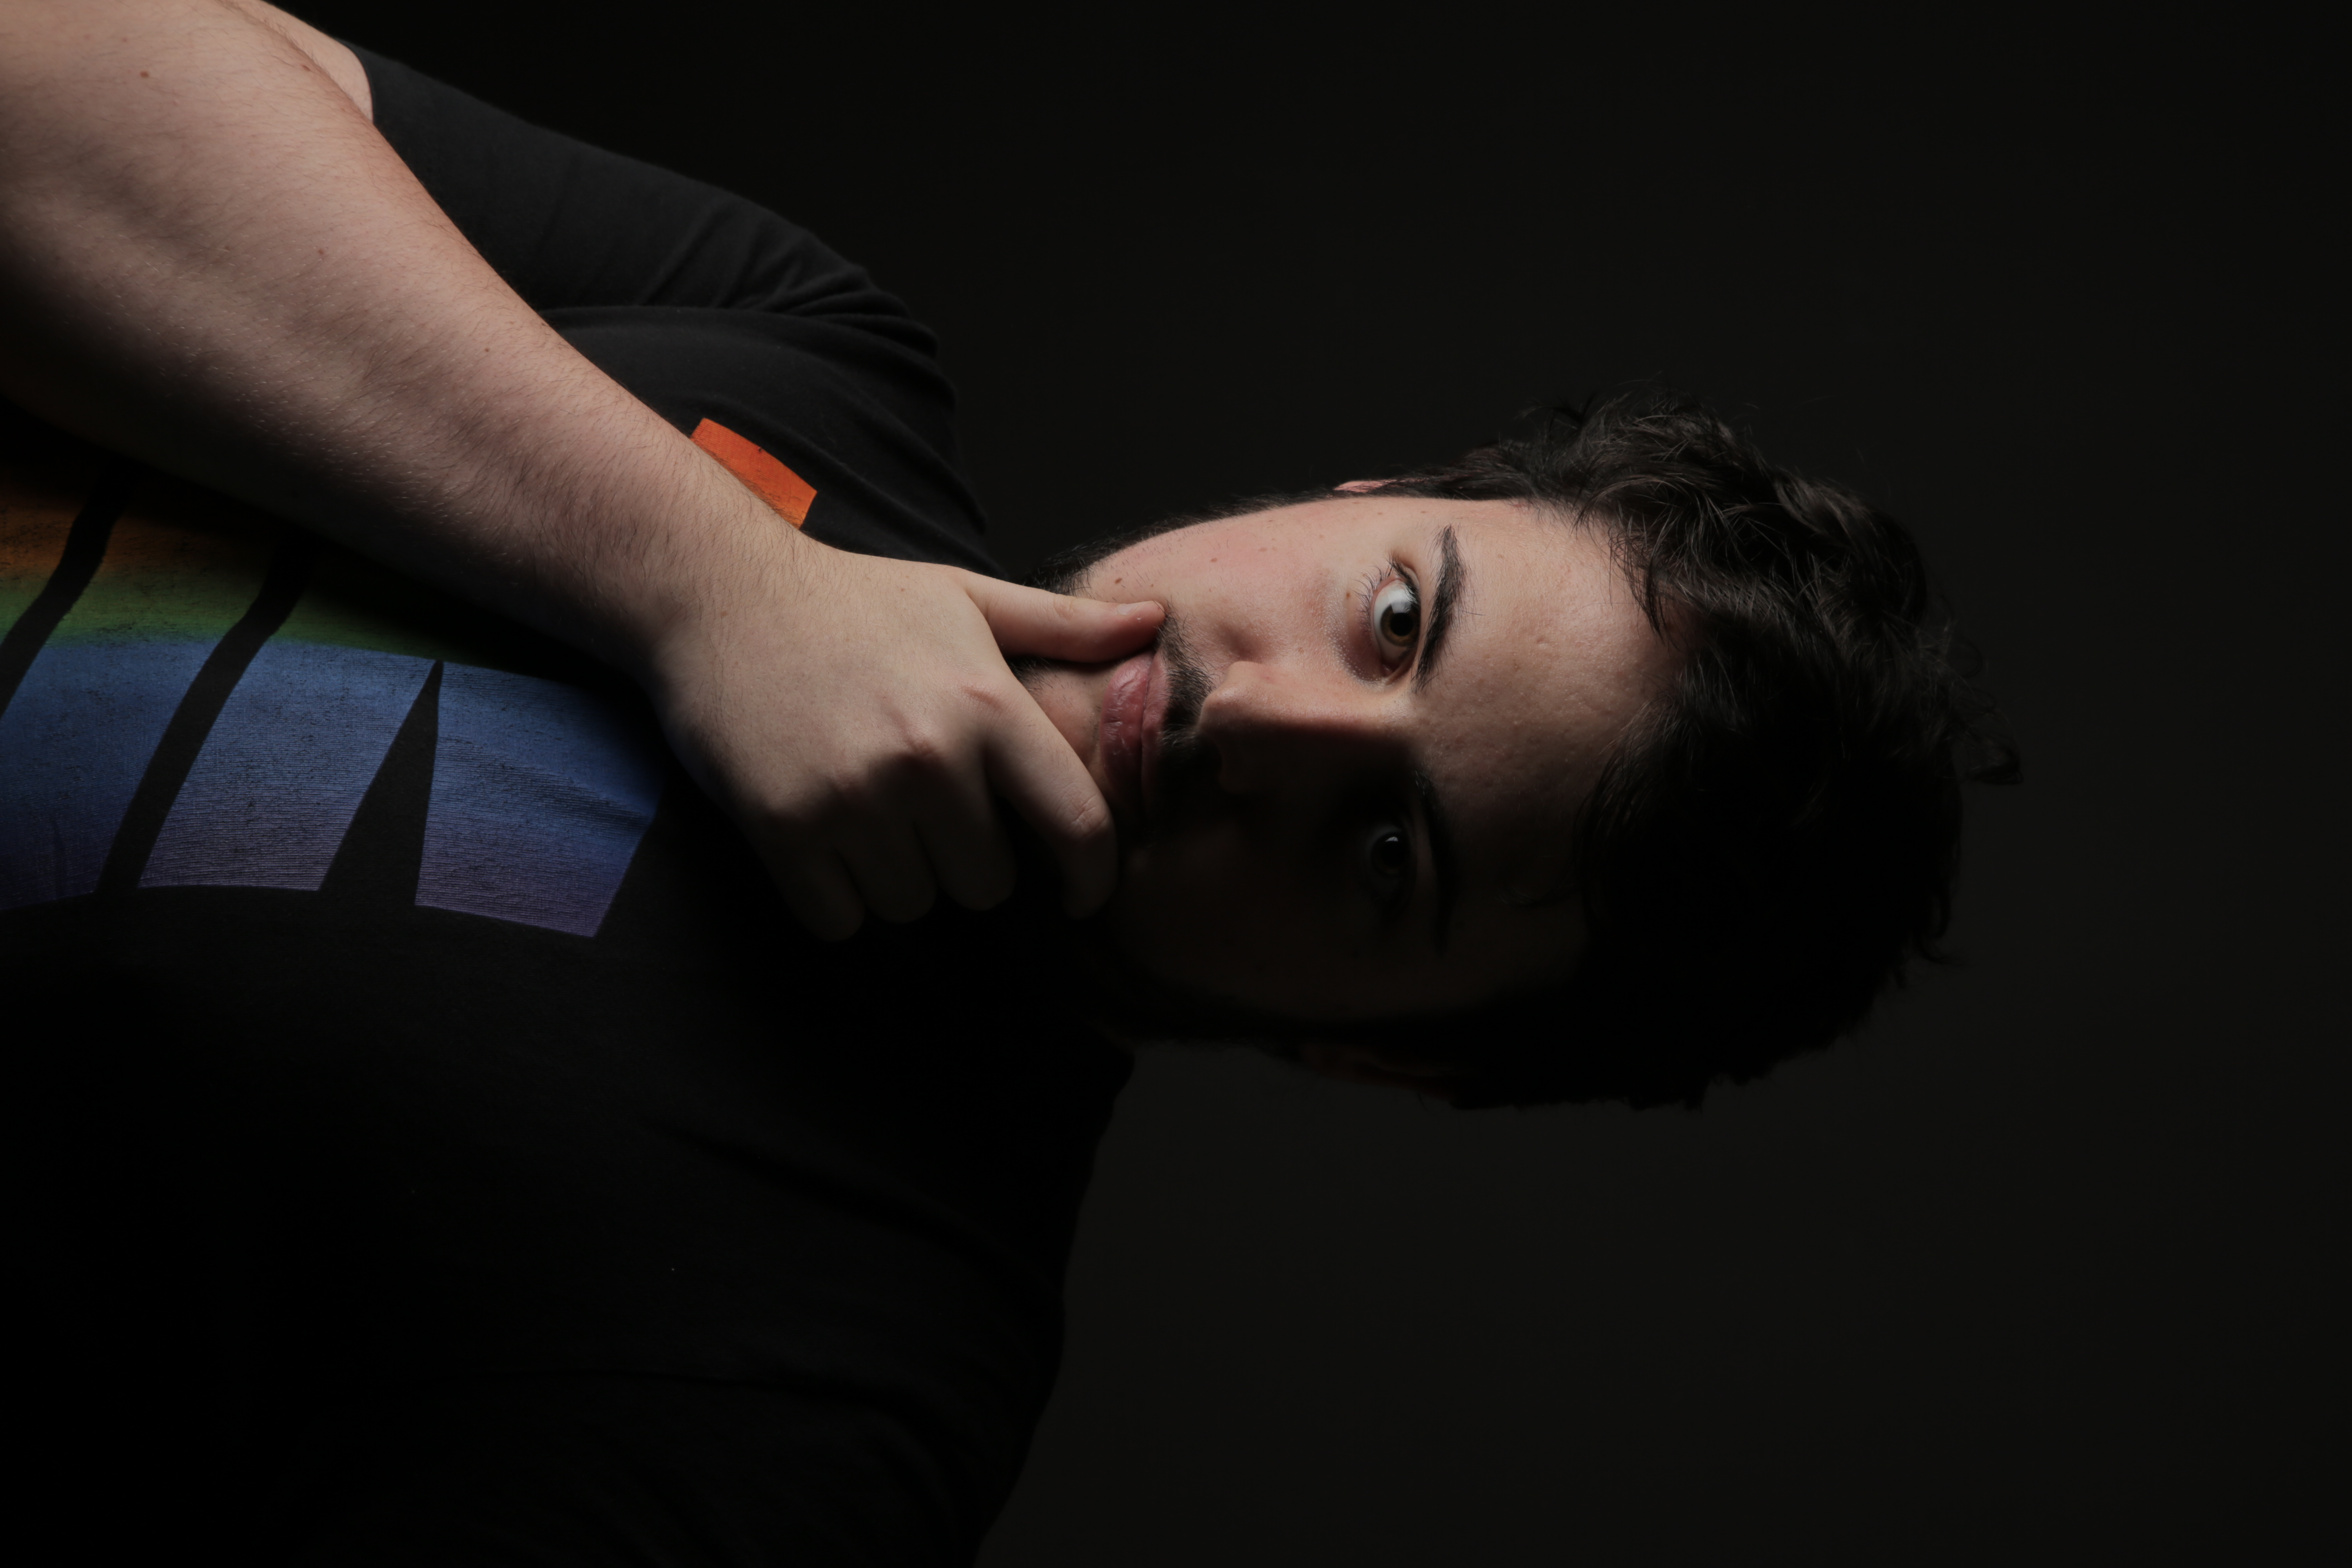
\includegraphics[height=6cm]{2-seitlich.jpg}
	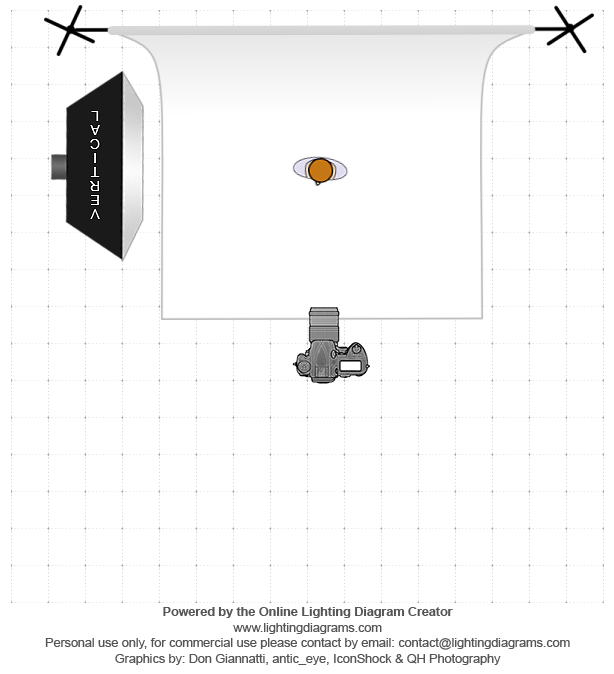
\includegraphics[height=5cm]{2-seitlich-diagram.png}
	\caption{Seitlich}
\end{figure}

Beim seitlichen Licht wird die Person nur von einer Seite ausgeleuchtet, während die andere im Dunkeln verschwindet. Dabei werden scharfe Schatten geworfen, welche Kanten betonen.
\\\\
Seitliches Licht wird häufig zur Betonung einer gespaltenen Persönlichkeit verwendet, Beispiele finden sich in Filmen des Regisseurs Martin Scorsese, wie etwa Shutter Island \cite{shutter-island}.
\section{Schurke}
\begin{figure}[h]
	\centering
	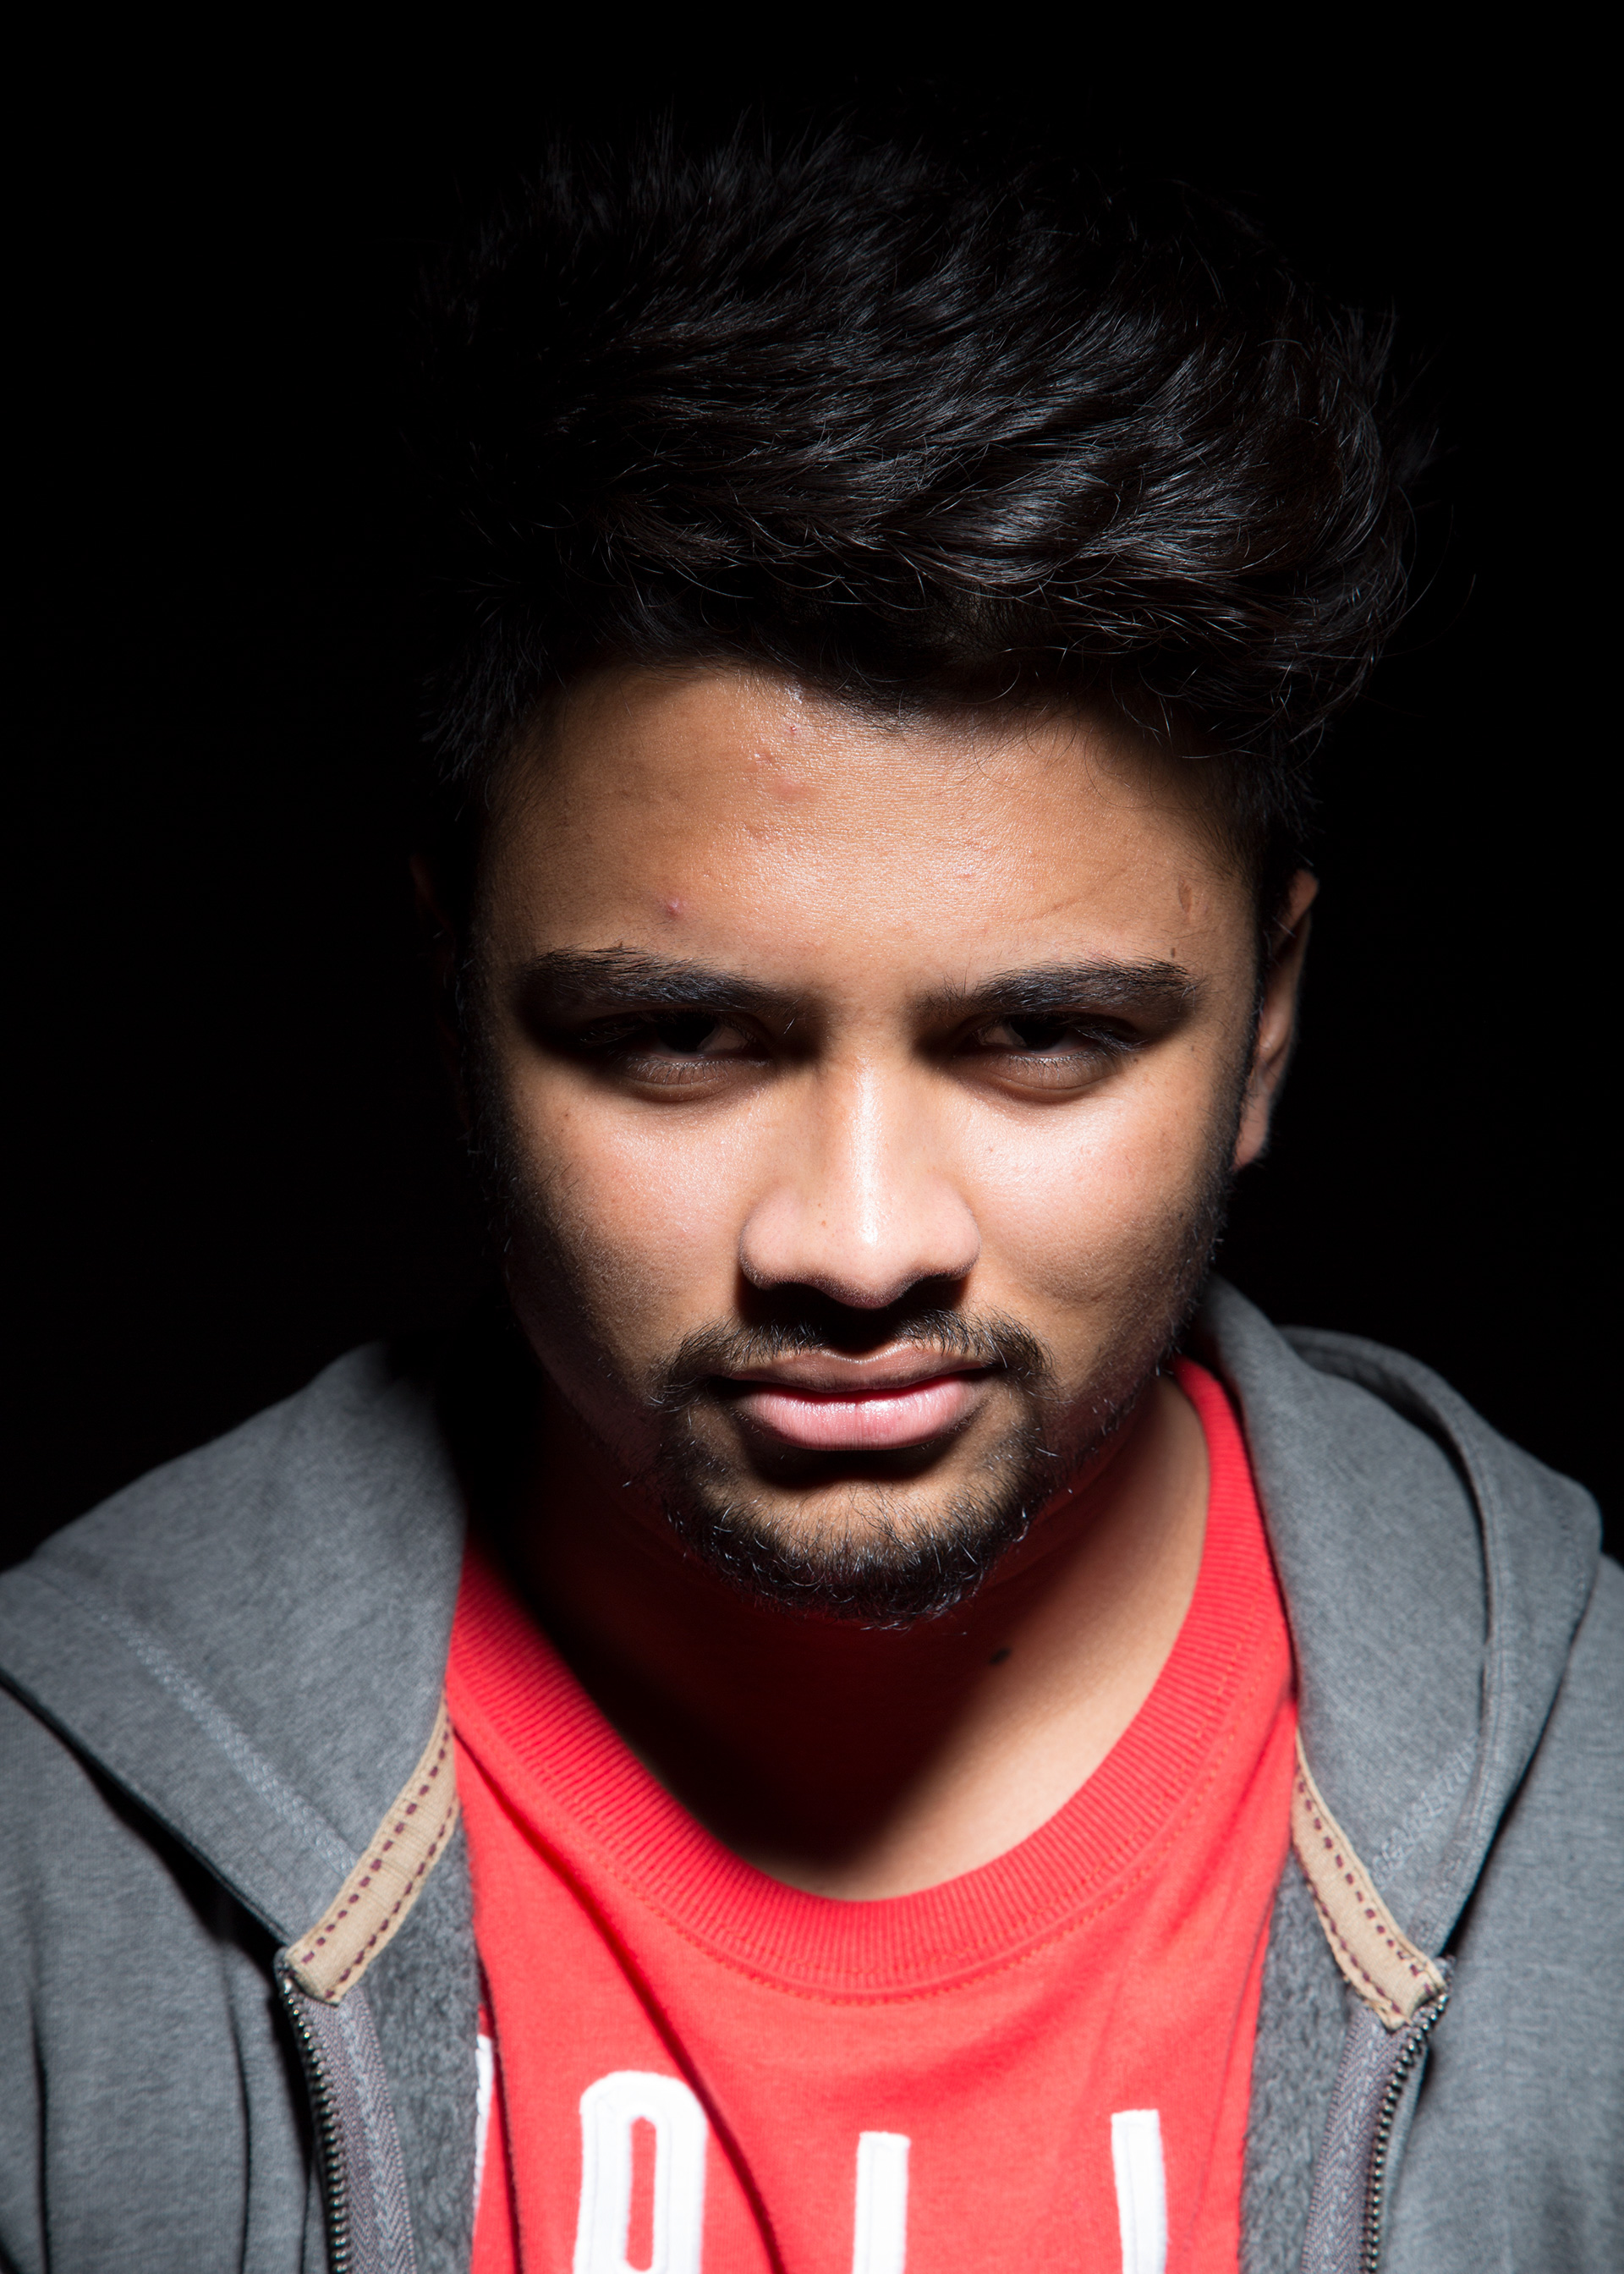
\includegraphics[height=6cm]{3-schurke.jpg}
	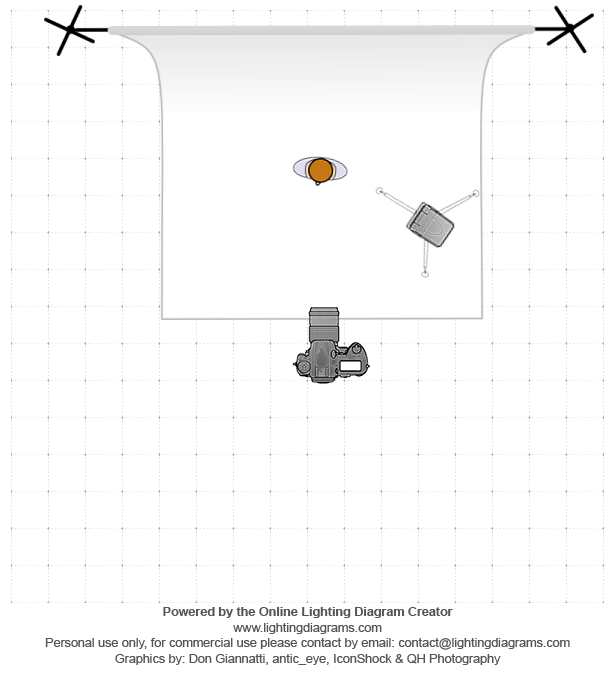
\includegraphics[height=5cm]{3-schurke-diagram.png}
	\caption{Schurke}
\end{figure}

Beim Schurkenlicht wird die Lichtquelle seitlich über der Person positioniert. Ziel ist es durch die Augenhöhlen, sowie die Nase und den Hals starke Schatten zu werfen.
\\\\
Das Schurkenlicht lässt die Person bedrohlich wirken, wodurch dieses gerne zur Darstellung von Antagonisten (Schurken) oder Gegnern des Protagonisten verwendet wird.

\newpage
\section{Totenkopf}
\begin{figure}[h]
	\centering
	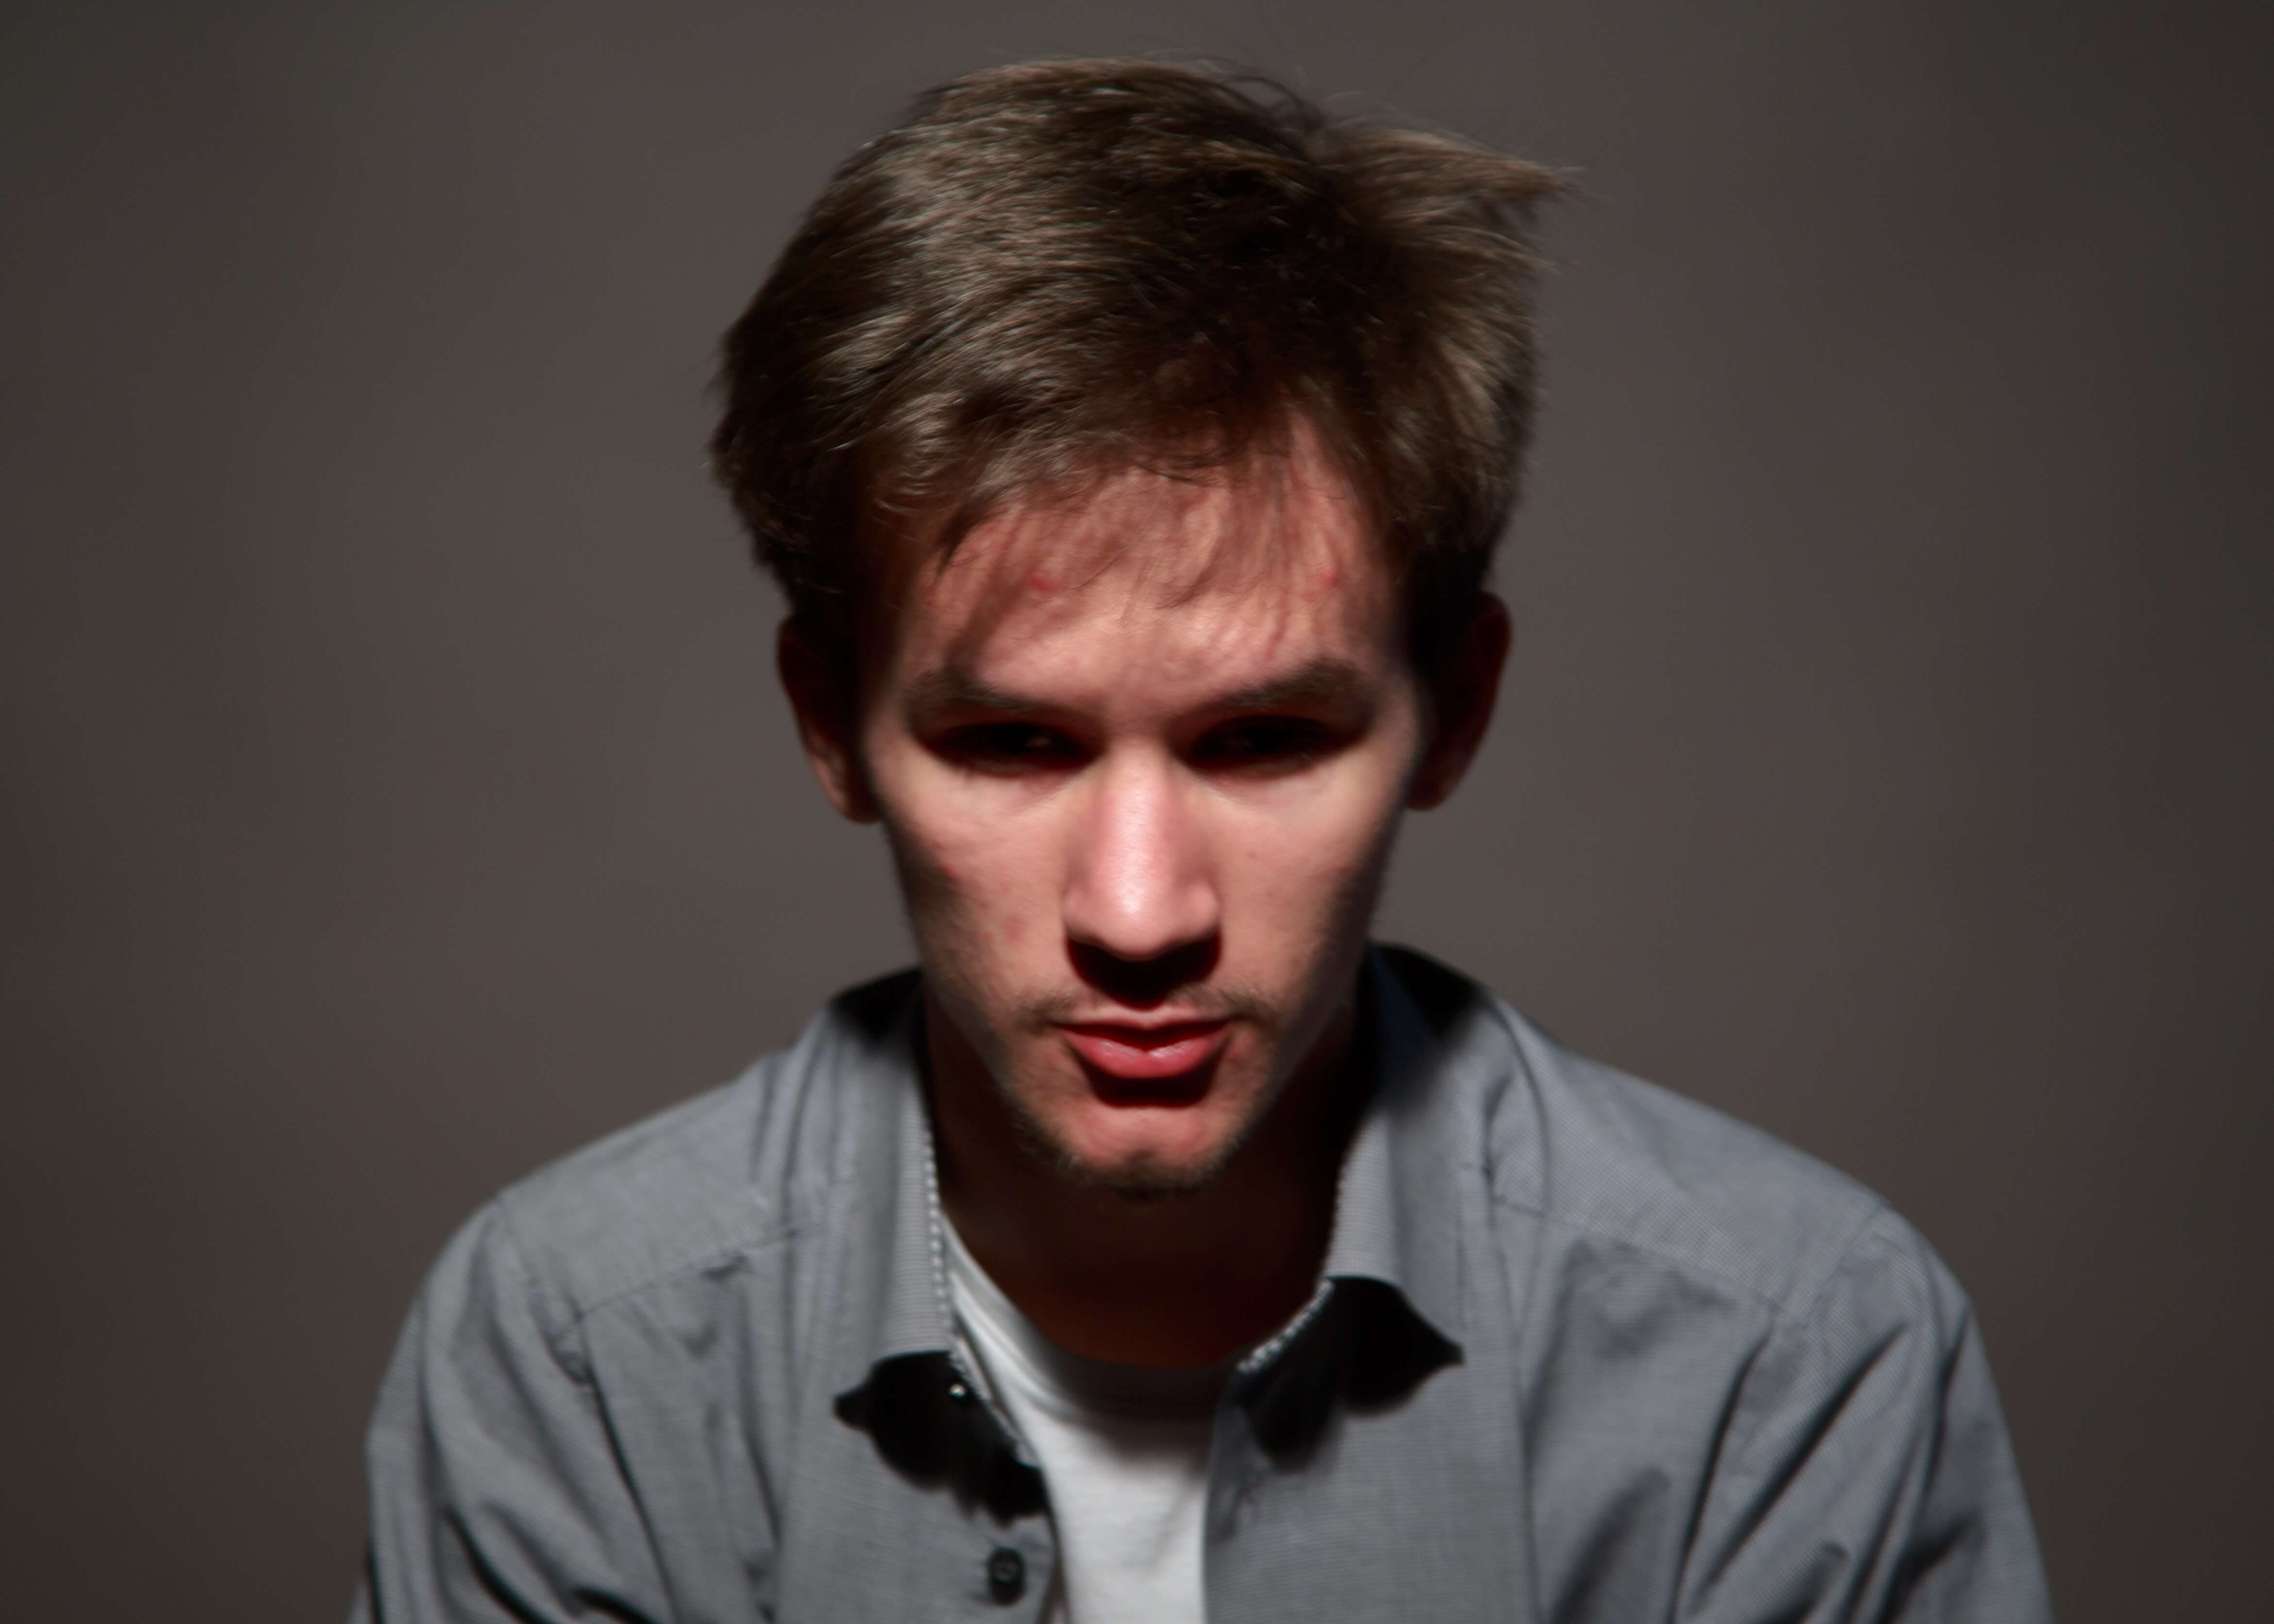
\includegraphics[height=5cm]{4-totenkopf.jpg}
	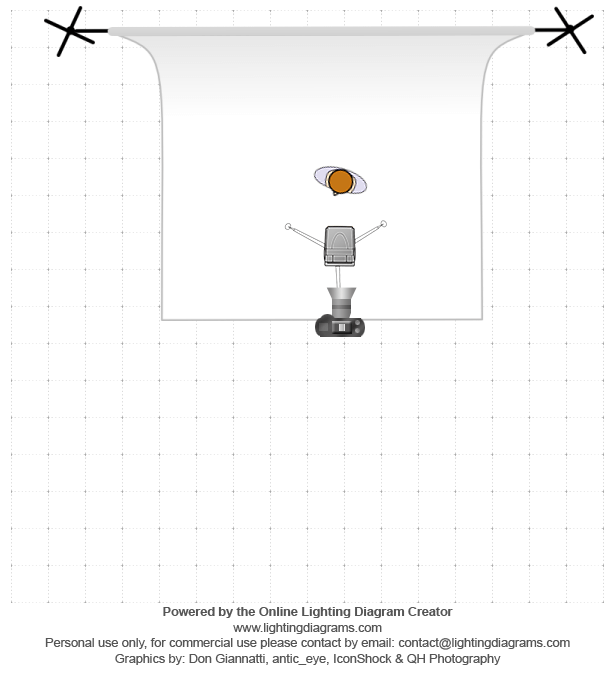
\includegraphics[height=5cm]{4-totenkopf-diagram.png}
	\caption{Totenkopf}
\end{figure}

Ein Totenkopflicht wird durch eine Lichtquelle über der Person erzeugt, wobei zusätzlich ein Aufheller verwendet werden kann um kein zu dunkles Bild zu erhalten.
\\\\
Knochen, Kanten und die Augenhöhlen werden besonders hervorgehoben, wodurch die Person mager oder gar krank erscheint. Beispiele finden sich etwa bei der Darstellung der fiktiven Figuren Gregory House \cite{gregory-house} und Walter White \cite{walter-white}, welche im Laufe ihrer Entwicklung immer stärker von schweren Krankheiten gezeichnet werden.

\section{Schmetterling}
\begin{figure}[h]
	\centering
	\includegraphics[height=6cm]{5-schmetterling.jpg}
	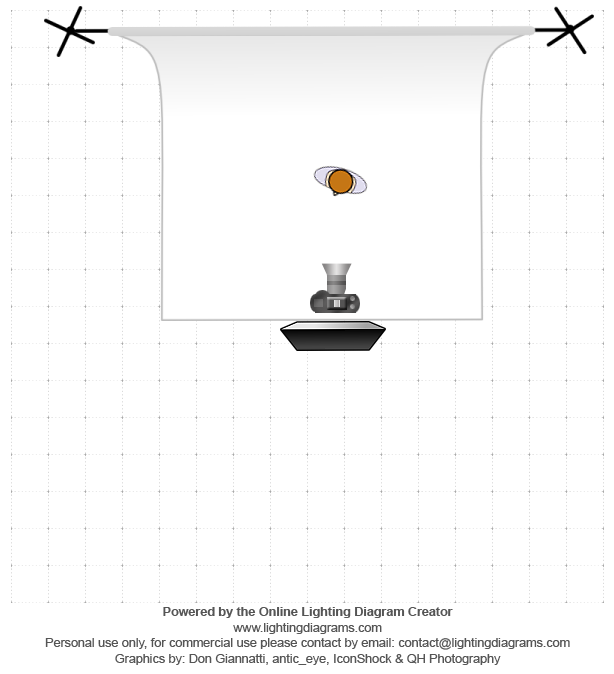
\includegraphics[height=5cm]{5-schmetterling-diagram.png}
	\caption{Schmetterling}
\end{figure}

Beim Schmetterlingslicht wird eine möglichst breite Lichtquelle (z.B.: Softbox) vor der Person und leicht über dem Kopf positioniert. Dadurch werden nur leichte Schatten geworfen, welche insbesondere zur Bildung eines "Schmetterlings" unterhalb der Nase führen.
\\\\
Die Lichtsetzung bildet eine Alternative zum schattenlosen Frontallicht

\newpage
\section{Frontal}
\begin{figure}[h]
	\centering
	\includegraphics[height=5cm]{6-frontal.jpg}
	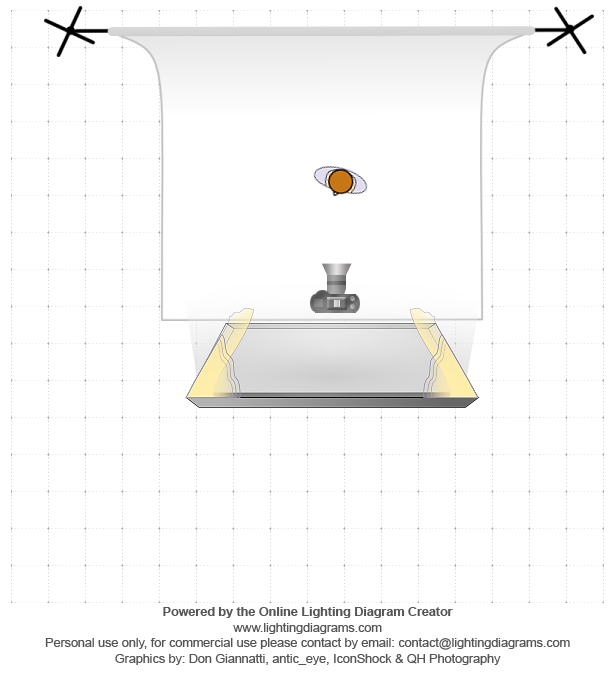
\includegraphics[height=5cm]{6-frontal-diagram.png}
	\caption{Frontal}
\end{figure}

Das Frontallicht wird besonders gerne für einfache Portraits, wie etwa Passfotos und Profilbilder verwendet, da es keine Schatten auf die Person selbst geworfen werden. Als Lichtquelle eignen sich neben einer Softbox auch Fenster oder bei einer Aufnahme im Freien sogar die Sonne. In geschlossenen Räumen sollte auch der Hintergrund ausgeleuchtet werden um Schatten auf Wänden und Objekten zu vermeiden.

\vfill{}

\listoffigures

\begin{thebibliography}{9}
\bibitem{fp-rembrandt} Fotopraxis.at, Das Rembrandt-Licht oder Dreiecks-Licht \\ https://www.fotopraxis.at/2010/12/03/das-rembrandt-licht-oder-dreiecks-licht/
\bibitem{shutter-island} Wikipedia, Shutter Island (Film) \\ https://de.wikipedia.org/wiki/Shutter\_Island\_(Film)
\bibitem{gregory-house} Wikipedia, Gregory House \\ https://en.wikipedia.org/wiki/Gregory\_House
\bibitem{walter-white} Wikipedia, Walter White (Breaking Bad) \\ https://en.wikipedia.org/wiki/Walter\_White\_(Breaking\_Bad)
\end{thebibliography}
\end{document}